\hypertarget{convolutional-coding}{%
\section{Convolutional Coding}\label{convolutional-coding}}

Bei den Blockcodes, kommen $k$ Nachrichten Bits rein und $n$ Code-Bits raus,
unabhängig davon was bereits vorher encoded wurde. Der Convolutional
Code hat nun aber ein Memory und dies beeinflusst die $n$ Code Bits.

Wie fest $n$ von $k$ abhängig ist kommt auf die sogenannte Rate drauf an.
Bei einer Rate von 1/2 kommt von einem $k$ Bit zwei $n$ Bit raus.

\begin{figure}[H]
\centering
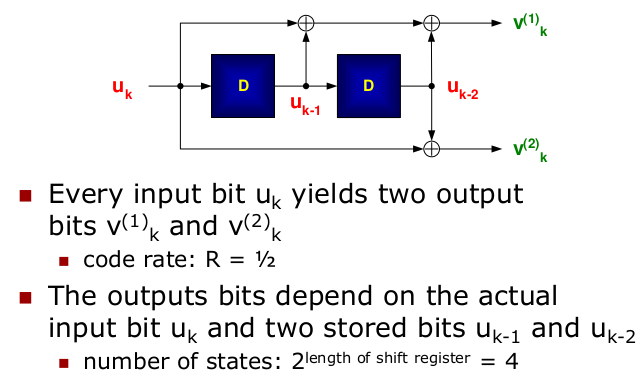
\includegraphics[width=0.6\textwidth]{figures/convolutional_example.png}
\caption{Example Block Diagram}
\end{figure}

\hypertarget{generator-sequences}{%
\subsection{Generator Sequences}\label{generator-sequences}}

Wenn man als Input eine einzelne 1, umgeben von alles 0, dann nennt man
dies eine \textbf{Impulsantwort}. Somit kann man schauen, wie sich die Ausgänge
verhalten.

\begin{itemize}
\tightlist
\item
  $g^1$ ist dabei die Generator-Sequenze die von als Impulsantwort am
  Ausgang $v^1$ generiert wird
\item
  $g^2$ gehört zum Ausgang $v^2$
\end{itemize}

\begin{figure}[H]
\centering
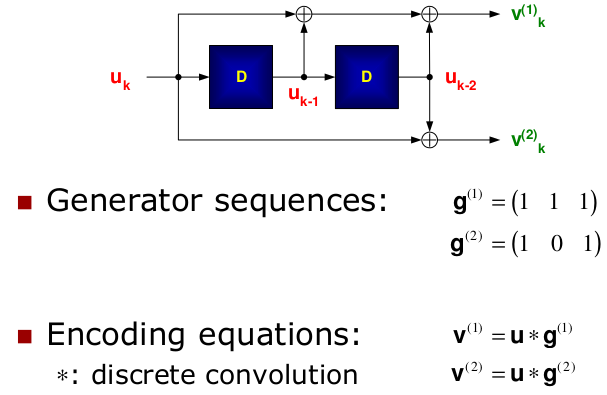
\includegraphics[width=0.5\textwidth]{figures/generator_sequences.png}
\caption{Generator Sequences}
\end{figure}

\hypertarget{polyonomial-representation}{%
\subsection{Polyonomial
Representation}\label{polyonomial-representation}}

\begin{figure}[H]
\centering
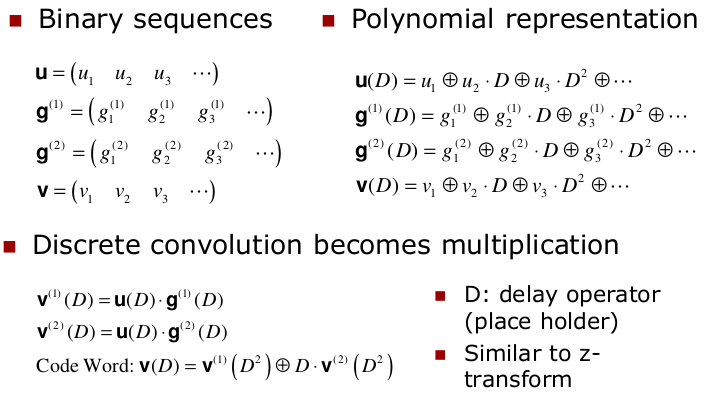
\includegraphics[width=0.5\textwidth]{figures/convolutional_polynomial.png}
\caption{Polynomial Representation}
\end{figure}

\hypertarget{encoder-state-diagram}{%
\subsection{Encoder State Diagram}\label{encoder-state-diagram}}

\begin{figure}[H]
\centering
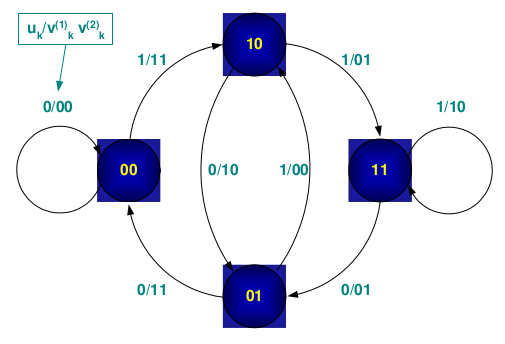
\includegraphics[width=0.5\textwidth]{figures/encoder_state_diagram.png}
\caption{Encoder State Diagram}
\end{figure}

\begin{itemize}
\tightlist
\item
  Wenn ich im Zustand $00$ starte, und es kommt eine $0$ rein, dann lande
  ich wieder im Zustand $00$. Dabei ist auch der Ausgang eine $00$
\item
  Wenn ich im Zustand $00$ bin und es kommt eine $1$ rein, dann wechsle ich
  in den Zustand $10$ und der Ausgang gibt $11$ raus.
\item
  Was uns hier fehlt ist die Zeit bzw. die Abfolge der Zustände
\end{itemize}

\hypertarget{treillis-diagram}{%
\subsection{Treillis Diagram}\label{treillis-diagram}}

\begin{figure}[H]
\centering
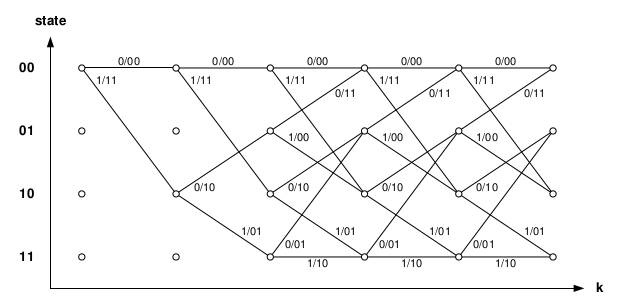
\includegraphics[width=0.5\textwidth]{figures/trellis_diagram.png}
\caption{Trellis Diagram}
\end{figure}

\begin{itemize}
\tightlist
\item
  Häufig ist es der Fall, dass man sagt dass man im Status $00$ startet
  und alle Speicher löscht
\item
  Dies ist aber nicht immer der Fall und es kann sein, dass man zu
  Beginn nicht weiss, in welchem Zustand man ist!
\item
  Manchmal fügt man am Schluss von ein paar gesendeten Bits wieder eine
  Anzahl $0$ an, damit der Ausgangszustand wieder $00$ ist.
\end{itemize}

\hypertarget{decoding-problem}{%
\subsection{Decoding Problem}\label{decoding-problem}}

\begin{itemize}
\tightlist
\item
  Die Aufgabe als Decoder besteht eigentlich darin, den bestmöglichen
  Weg im Trellis Diagramm zu finden, den zu den Bits passt, die ich
  empfangen habe.
\item
  Hard decoding

  \begin{itemize}
  \tightlist
  \item
    Der Empfänger sendet ein binäres Symbol
  \item
    Man entscheidet anhand der Hamming Distanz zwischen den empfangenen
    Bits und den Pfäden im Diagramm
  \end{itemize}
\item
  Soft decoding

  \begin{itemize}
  \tightlist
  \item
    Der Empfänger sendet eine Floating Point Zahl
  \item
    Jetzt ist wichtig, um wie viel unterscheiden die Werte sich
  \item
    Squared Euclidean Distance $(r - v)^2$, also empfangene Bits - Pfad
    hoch 2
  \item
    Ist 2 dB besser als Hard decoding
  \end{itemize}
\end{itemize}

\hypertarget{viterbi-algorithm}{%
\subsection{Viterbi Algorithm}\label{viterbi-algorithm}}

\begin{itemize}
\tightlist
\item
  Findet den Pfad durch das Trellis Diagramm mit der grössten (oder der
  kleinsten) Metrik
\item
  Vorgehen

  \begin{itemize}
  \tightlist
  \item
    In jedem Schritt vergleicht man alle Metriken, die zum aktuellen
    Pfad hinführen. Man speichert den Pfad mit der grössten Metrik und
    löscht alle anderen Pfade
  \item
    Am Schluss wird der beste Pfad gewählt (mit der besten Metrik) und
    die Bits auf diesem Pfad sind dann die dekodierten Bits
  \end{itemize}
\end{itemize}

\begin{figure}[H]
\centering
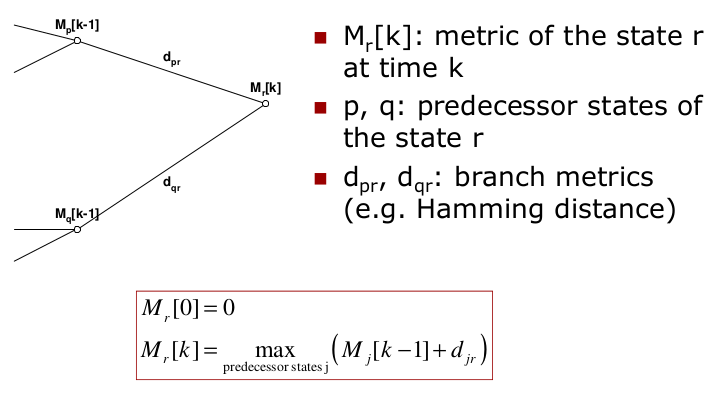
\includegraphics[width=0.4\textwidth]{figures/viterbi_algorithm.png}
\caption{Viterbi Algorithm}
\end{figure}

\begin{figure}[H]
\centering
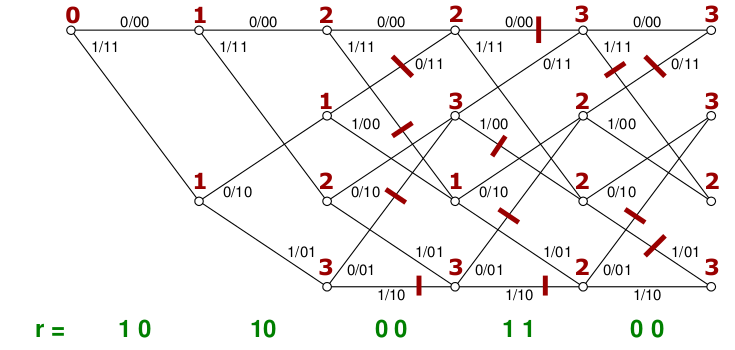
\includegraphics[width=0.5\textwidth]{figures/viterbi_example.png}
\caption{Example}
\end{figure}

\begin{itemize}
\tightlist
\item
  Wenn wir im $00$ starten und $01$ erhalten, berechnen wir die Hamming
  Distanz zu den folgenden Punkten und schreiben sie hin (in beiden
  Fällen 1)
\item
  Dann erhalten wir $10$ und berechnen wieder von beiden möglichen
  Zuständen die Hamming Distanz
\item
  Dies machen wir sicher, bis wir alle möglichen Bit-Zustände erreicht
  haben
\item
  Ab dann können wir beginnen Pfäde rauszustreichen, z.B.

  \begin{itemize}
  \tightlist
  \item
    Wir sind beim dritten Schritt und erhalten $00$
  \item
    Das heisst entweder waren wir vorher bei $0/00$ oder $0/11$
  \item
    Da die Metrik für $0/11$ nachher bei $00$ schlechter ist, streichen wir
    diesen Pfad und gehen mit $0/00$
  \end{itemize}
\item
  Falls ich Pfade habe, die dieselbe Metrik haben, muss ich trotzdem
  eine streichen. Zufallsprinzip!
\item
  Irgendwann muss man sich für einen Pfad entscheiden. Dies ist optimal
  am Schluss, kann aber auch oft schon früher sein, da die
  Bit-Reihenfolgen zu lang werden
\item
  Der Zustand mit der kleinsten Metrik-Angabe ist der ``Winner-State''.
\item
  Vom Winner-State führt nun ein eindeutiger Pfad zum Ausgangspunkt
  zurück
\end{itemize}

\clearpage
